% !TEX TS-program = xelatex
% !BIB program = bibtex
% !TeX spellcheck = ru_RU
% !TEX root = talk.tex

\documentclass
  [ russian
  , aspectratio=1610 % Для защит онлайн лучше использовать разрешение не 4х3
  ] {beamer}


% !TeX spellcheck = ru_RU
% !TEX root = vkr.tex
% Опциональные добавления используемых пакетов. Вполне может быть, что они вам не понадобятся, но в шаблоне приведены примеры их использования.
\usepackage{tikz} % Мощный пакет для создание рисунков, однако может очень сильно замедлять компиляцию
\usetikzlibrary{decorations.pathreplacing,calc,shapes,positioning,tikzmark}

% Библиотека для TikZ, которая генерирует отдельные файлы для каждого рисунка
% Позволяет ускорить компиляцию, однако имеет свои ограничения
% Например, ломает пример выделения кода в листинге из шаблона
% \usetikzlibrary{external}
% \tikzexternalize[prefix=figures/]

\newcounter{tmkcount}

\tikzset{
    use tikzmark/.style={
            remember picture,
            overlay,
            execute at end picture={
                    \stepcounter{tmkcount}
                },
        },
    tikzmark suffix={-\thetmkcount}
}

\usepackage{booktabs} % Пакет для верстки "более книжных" таблиц, вполне годится для оформления результатов
% В шаблоне есть команда \multirowcell, которой нужен этот пакет.
\usepackage{multirow}
\usepackage{siunitx} % для таблиц с единицами измерений

% Для названий стоит использовать \textsc{}
\newcommand{\OCaml}{\textsc{OCaml}}
\newcommand{\miniKanren}{\textsc{miniKanren}}
\newcommand{\BibTeX}{\textsc{BibTeX}}
\newcommand{\vsharp}{\textsc{V$\sharp$}}
\newcommand{\fsharp}{\textsc{F$\sharp$}}
\newcommand{\csharp}{\textsc{C\#}}
\newcommand{\GitHub}{\textsc{GitHub}}
\newcommand{\SMT}{\textsc{SMT}}

\definecolor{eclipseGreen}{RGB}{63,127,95}
% \lstdefinelanguage{ocaml}{
% keywords={@type, function, fun, let, in, match, with, when, class, type,
% nonrec, object, method, of, rec, repeat, until, while, not, do, done, as, val, inherit, and,
% new, module, sig, deriving, datatype, struct, if, then, else, open, private, virtual, include, success, failure,
% lazy, assert, true, false, end},
% sensitive=true,
% commentstyle=\small\itshape\ttfamily,
% keywordstyle=\ttfamily\bfseries, %\underbar,
% identifierstyle=\ttfamily,
% basewidth={0.5em,0.5em},
% columns=fixed,
% fontadjust=true,
% literate={->}{{$\to$}}3 {===}{{$\equiv$}}1 {=/=}{{$\not\equiv$}}1 {|>}{{$\triangleright$}}3 {\\/}{{$\vee$}}2 {/\\}{{$\wedge$}}2 {>=}{{$\ge$}}1 {<=}{{$\le$}} 1,
% morecomment=[s]{(*}{*)}
% }

\makeatletter
\@ifclassloaded{beamer}{
    %%% Обязательные пакеты
    %% Beamer
    \usepackage{beamerthemesplit}
    \usetheme{SPbGU}
    \beamertemplatenavigationsymbolsempty
    \usepackage{appendixnumberbeamer}

    %% Локализация
    \usepackage{fontspec}
    \setmainfont{CMU Serif}
    \setsansfont{CMU Sans Serif}
    \setmonofont{CMU Typewriter Text}
    %\setmonofont{Fira Code}[Contextuals=Alternate,Scale=0.9]
    %\setmonofont{Inconsolata}
    \usepackage{polyglossia}
    \setmainlanguage{russian}
    \setotherlanguage{english}

    %% Графика
    \usepackage{pdfpages} % Позволяет вставлять многостраничные pdf документы в текст

    % Математические окружения с русским названием
    \newtheorem{rutheorem}{Теорема}
    \newtheorem{ruproof}{Доказательство}
    \newtheorem{rudefinition}{Определение}
    \newtheorem{rulemma}{Лемма}
    \usepackage{fancyvrb}
}
{}
\makeatother

\usepackage[autostyle]{csquotes} % Правильные кавычки в зависимости от языка
\usepackage{totcount}
\usepackage{setspace}
\usepackage{amsmath, amsfonts, amssymb, amsthm, mathtools} % "Адекватная" работа с математикой в LaTeX


\makeatletter

%!TEX root = vkr.tex

%% Параметры заполнения титульного листа
\usepackage{xkeyval}

%% Русскоязычный вариант
\define@key[ru]{mytitle}{chair}{\def\my@title@chair@ru{#1}}
\define@key[ru]{mytitle}{title}{\def\my@title@title@ru{#1}}
\define@key[ru]{mytitle}{group}{\def\my@title@group@ru{#1}}
\define@key[ru]{mytitle}{author}{\def\my@title@author@ru{#1}}
\define@key[ru]{mytitle}{supervisor}{\def\my@title@supervisor@ru{#1}}
\define@key[ru]{mytitle}{supervisorPosition}{\def\my@title@supervisorPosition@ru{#1}}
\define@key[ru]{mytitle}{reviewer}{\def\my@title@reviewer@ru{#1}}
\define@key[ru]{mytitle}{reviewerPosition}{\def\my@title@reviewerPosition@ru{#1}}
\define@key[ru]{mytitle}{consultant}{\def\my@title@consultant@ru{#1}}
\define@key[ru]{mytitle}{consultantPosition}{\def\my@title@consultantPosition@ru{#1}}
\define@key[ru]{mytitle}{year}{\def\my@title@year@ru{#1}}
\define@key[ru]{mytitle}{specialty}{\def\my@title@specialty@ru{#1}}
\define@key[ru]{mytitle}{programme}{\def\my@title@programme@ru{#1}}
\define@key[ru]{mytitle}{profile}{\def\my@title@profile@ru{#1}}
\define@choicekey*[ru]{mytitle}{type}{coursework,practice,prediploma,master,bachelor,production}{\def\my@title@type@ru{#1}}
\define@choicekey*[ru]{mytitle}{kind}{solution,experiment,production,comparison,theoretical}{\def\my@title@kind@ru{#1}}

%% Англоязычный вариант
\define@key[en]{mytitle}{chair}{\def\my@title@chair@en{#1}}
\define@key[en]{mytitle}{title}{\def\my@title@title@en{#1}}
\define@key[en]{mytitle}{group}{\def\my@title@group@en{#1}}
\define@key[en]{mytitle}{author}{\def\my@title@author@en{#1}}
\define@key[en]{mytitle}{supervisor}{\def\my@title@supervisor@en{#1}}
\define@key[en]{mytitle}{supervisorPosition}{\def\my@title@supervisorPosition@en{#1}}
\define@key[en]{mytitle}{reviewer}{\def\my@title@reviewer@en{#1}}
\define@key[en]{mytitle}{reviewerPosition}{\def\my@title@reviewerPosition@en{#1}}
\define@key[en]{mytitle}{consultant}{\def\my@title@consultant@en{#1}}
\define@key[en]{mytitle}{consultantPosition}{\def\my@title@consultantPosition@en{#1}}
\define@key[en]{mytitle}{year}{\def\my@title@year@en{#1}}
\define@key[en]{mytitle}{specialty}{\def\my@title@specialty@en{#1}}
\define@key[en]{mytitle}{programme}{\def\my@title@programme@en{#1}}
\define@key[en]{mytitle}{profile}{\def\my@title@profile@en{#1}}
\define@choicekey*[en]{mytitle}{type}{coursework,practice,prediploma,master,bachelor}{\def\my@title@type@en{#1}}
\define@choicekey*[en]{mytitle}{kind}{solution,experiment,production,comparison,theoretical}{\def\my@title@kind@en{#1}}

\newcommand{\filltitle}[2]{
    %% Значения по умолчанию для обоих языков
    \ifthenelse{\equal{#1}{ru}}
    {
        \presetkeys[#1]{mytitle}{
            year = {\the\year},
            type = {practice},
            reviewer = {},
            consultant = {},
            profile = {}
        }{}
    }
    {}
    \ifthenelse{\equal{#1}{en}}
    {
        \presetkeys[#1]{mytitle}{
            year = {\the\year},
            type = {practice},
            reviewer = {},
            consultant = {},
            profile = {}
        }{}
    }
    {}
    \setkeys[#1]{mytitle}{#2}
}


% !TeX spellcheck = ru_RU
% !TEX root = vkr.tex

%% Если что-то забыли, при компиляции будут ошибки Undefined control sequence \my@title@<что забыли>@ru
%% Если англоязычная титульная страница не нужна, то ее можно просто удалить.
\filltitle{ru}{
    %% Актуально только для курсовых/практик. ВКР защищаются не на кафедре а в ГЭК по направлению,
    %%   и к моменту защиты вы будете уже не в группе.
    chair              = {Кафедра информатики},
    group              = {23.Б16-мм},
    %
    %% Макрос filltitle ненавидит пустые строки, поэтому обязателен хотя бы символ комментария на строке
    %% Актуально всем.
    title              = {Реализация и внедрение архитектуры Gated Recurrent Unit в пакет DEGANN \cite{degann}},
    %
    %% Здесь указывается тип работы. Возможные значения:
    %%   production - производственная практика;
    %%   coursework - отчёт по курсовой работе (ОБРАТИТЕ ВНИМАНИЕ, у техпрога и ПИ нет курсовых, только практики);
    %%   practice - отчёт по учебной практике;
    %%   prediploma - отчёт по преддипломной практике;
    %%   master - ВКР магистра;
    %%   bachelor - ВКР бакалавра.
    type               = {practice},
    %
    %% Здесь указывается вид работы. От вида работы зависят критерии оценивания.
    %%   solution - «Решение». Обучающемуся поручили найти способ решения проблемы в области разработки программного обеспечения или теоретической информатики с учётом набора ограничений.
    %%   experiment - «Эксперимент». Обучающемуся поручили изучить возможности, достоинства и недостатки новой технологии, платформы, языка и т. д. на примере какой-то задачи.
    %%   production - «Производственное задание». Автору поручили реализовать потенциально полезное программное обеспечение.
    %%   comparison - «Сравнение». Обучающемуся поручили сравнить несколько существующих продуктов и/или подходов.
    %%   theoretical - «Теоретическое исследование». Автору поручили доказать какое-то утверждение, исследовать свойства алгоритма и т.п., при этом не требуя написания кода.
    kind               = {production},
    %
    author             = {Мурадян Денис Степанович},
    %
    %% Актуально только для ВКР. Указывается код и название направления подготовки. Типичные примеры:
    %%   02.03.03 \enquote{Математическое обеспечение и администрирование информационных систем}
    %%   02.04.03 \enquote{Математическое обеспечение и администрирование информационных систем}
    %%   09.03.04 \enquote{Программная инженерия}
    %%   09.04.04 \enquote{Программная инженерия}
    %% Те, что с 03 в середине --- бакалавриат, с 04 --- магистратура.
    specialty          = {02.03.03 \enquote{Математическое обеспечение и администрирование информационных систем}},
    %
    %% Актуально только для ВКР. Указывается шифр и название образовательной программы. Типичные примеры:
    %%   СВ.5162.2020 \enquote{Технологии программирования}
    %%   СВ.5080.2020 \enquote{Программная инженерия}
    %%   ВМ.5665.2022 \enquote{Математическое обеспечение и администрирование информационных систем}
    %%   ВМ.5666.2022 \enquote{Программная инженерия}
    %% Шифр и название программы можно посмотреть в учебном плане, по которому вы учитесь.
    %% СВ.* --- бакалавриат, ВМ.* --- магистратура. В конце --- год поступления (не обязательно ваш, если вы были в академе/вылетали).
    programme          = {СВ.5162.2020 \enquote{Технологии программирования}},
    %
    %% Актуально всем.
    %% Должно умещаться в одну строчку, допускается использование сокращений, но без переусердствования,
    %% короткая строка с большим количеством сокращений выглядит странно
    %supervisorPosition = {проф. кафeдры системного программирования, д.ф.-м.н.,}, % Терехов А. Н.
    %supervisorPosition = {ст. преподаватель кафедры ИАС, к.~ф.-м.~н. (если есть),}, % Смирнов К. К.
    supervisorPosition = {доцент кафедры ситемного программирования, к.ф.-м.н.,},
    supervisor         = {Гориховский~В.~И.},
    %
    %% Актуально только для практик и курсовых. Если консультанта нет или он совпадает с научником, закомментировать или удалить вовсе.
    consultantPosition = {Преподаватель СПбГУ,},
    consultant         = {Алимов~П.~Г.},
}

% Английский титульник нужен только для ВКР, остальные виды работ могут его смело игнорировать.
\filltitle{en}{
    chair              = {Advisor's chair},
    group              = {ХХ.BХХ-mm},
    title              = {Template for SPbU qualification works},
    type               = {bachelor},
    author             = {FirstName Surname},
    %
    %% Possible choices:
    %%   02.03.03 \foreignquote{english}{Software and Administration of Information Systems}
    %%   02.04.03 \foreignquote{english}{Software and Administration of Information Systems}
    %%   09.03.04 \foreignquote{english}{Software Engineering}
    %%   09.04.04 \foreignquote{english}{Software Engineering}
    %% Те, что с 03 в середине --- бакалавриат, с 04 --- магистратура.
    specialty          = {02.03.03 \foreignquote{english}{Software and Administration of Information Systems}},
    %
    %% Possible choices:
    %%   СВ.5162.2020 \foreignquote{english}{Programming Technologies}
    %%   СВ.5080.2020 \foreignquote{english}{Software Engineering}
    %%   ВМ.5665.2022 \foreignquote{english}{Software and Administration of Information Systems}
    %%   ВМ.5666.2022 \foreignquote{english}{Software Engineering}
    programme          = {СВ.5162.2020 \foreignquote{english}{Programming Technologies}},
    %
    %% Note that common title translations are:
    %%   кандидат наук --- C.Sc. (NOT Ph.D.)
    %%   доктор ... наук --- Sc.D.
    %%   доцент --- docent (NOT assistant/associate prof.)
    %%   профессор --- prof.
    supervisorPosition = {Sc.D, prof.},
    supervisor         = {S.S. Supervisor},
    %
    consultantPosition = {position at \foreignquote{english}{Company}, degree if present},
    consultant         = {C.C. Consultant},
    %
    reviewerPosition   = {position at \foreignquote{english}{Company}, degree if present},
    reviewer           = {R.R. Reviewer},
}


\newcommand{\academicGroup}{\my@title@group@ru}
\newcommand{\advisorChair}{\my@title@chair@ru}
% То, что в квадратных скобках, отображается внизу по центру каждого слайда.
\title[GRU в DEGANN]{\my@title@title@ru}
% То, что в квадратных скобках, отображается в левом нижнем углу.
\author[\my@title@author@ru]{\my@title@author@ru, группа \academicGroup}
\institute[СПбГУ]{}
\date[10 декабря 2024 г.]{}
\newcommand{\supervisor}{\my@title@supervisor@ru}
\newcommand{\supervisorPosition}{\my@title@supervisorPosition@ru}
\newcommand{\consultant}{\my@title@consultant@ru}
\newcommand{\consultantPosition}{\my@title@consultantPosition@ru}
\newcommand{\reviewer}{\my@title@reviewer@ru}
\newcommand{\reviewerPosition}{\my@title@reviewerPosition@ru}
\newcommand{\defenseYear}{\my@title@year@ru}

\makeatother
\begin{document}
{
\setbeamertemplate{footline}{}
% Лого университета или организации, отображается в шапке титульного листа
\begin{frame}
    
\includegraphics[width=1.4cm]{figures/SPbGU_Logo.png}
    \vspace{-35pt}
    \hspace{-10pt}
    \begin{center}
        \begin{tabular}{c}
            \scriptsize{Санкт-Петербургский государственный университет} \\
            \scriptsize{\advisorChair}
        \end{tabular}
        \titlepage
    \end{center}

    \btVFill

    {\scriptsize
        % У научного руководителя должна быть указана научная степень
        \textbf{Научный руководитель:}  \supervisorPosition~\supervisor \\
        % Консультанта может и не быть. Должна быть указана должность или ученая степень
        \textbf{Консультант:}  \consultantPosition~\consultant \\
    }
    \makeatother
    \begin{center}
        \vspace{5pt}
        \scriptsize{Санкт-Петербург\\ \defenseYear}
    \end{center}
\end{frame}
}

\begin{frame}{Введение}
    \begin{itemize}
        \item Дифференциальные уравнения широко применяются в науке и технике
        \item Традиционные численные методы сталкиваются с проблемами, связанными с длительным вычислением и недостаточной точностью
        \item Библиотека для нейросетевой аппроксимации дифференциальных уравнений
        \item Цель работы: интеграция архитектуры GRU в DEGANN
    \end{itemize}
\end{frame}

\begin{frame}
    \frametitle{Архитектура и принцип работы GRU}
    \begin{itemize}
        \item \textbf{RNN (Recurrent Neural Networks):}
        \begin{itemize}
            \item Преимущества: используют скрытые состояния для учёта временных зависимостей.
            \item Проблемы: затухание и взрыв градиентов, затрудняющие обучение на длинных последовательностях.
        \end{itemize}
        \item \textbf{GRU (Gated Recurrent Unit):}
        \begin{itemize}
            \item обновляющий (\( z_t \)) и сбрасывающий (\( r_t \)) гейты:
            \[
            z_t = \sigma(W_z \cdot [h_{t-1}, x_t] + b_z), \quad
            r_t = \sigma(W_r \cdot [h_{t-1}, x_t] + b_r)
            \]
            \item Новое состояние:
            \[
            h_t = z_t \odot h_{t-1} + (1 - z_t) \odot \tilde{h}_t, \quad
            \tilde{h}_t = \tanh(W_h \cdot [r_t \odot h_{t-1}, x_t] + b_h)
            \]
        \end{itemize}
        \item \textbf{Преимущества GRU:}
        \begin{itemize}
            \item Сохраняет зависимость в последовательности данных
            \item Частично решает затухание градиентов, учитывая долгосрочные зависимости.
            \item Компактная структура.
        \end{itemize}
    \end{itemize}
\end{frame}


\begin{frame}
    \frametitle{Рекуррентные слои в TensorFlow}
    \begin{itemize}
        \item \textbf{Использование TensorFlow:}
        \begin{itemize}
            \item Для реализации GRU использовался встроенный слой \texttt{tf.keras.layers.GRU}.
            \item Слой предоставляет механизмы управления потоками данных:
            \begin{itemize}
                \item Обновляющий и сбрасывающий гейты.
                \item Поддержка скрытых состояний.
            \end{itemize}
            \item Интеграция GRU с TensorFlow позволяет сосредоточиться на настройке модели и анализе её поведения, а так же настройке гиперпараметров.
        \end{itemize}
        \item \textbf{Существующая проблема:}
        \begin{itemize}
            \item Текущая версия DEGANN имеет только полносвязные сети, что ограничивает возможности аппроксимации сложных функций.
        \end{itemize}
        \item \textbf{Выводы:}
        \begin{itemize}
            \item GRU может помочь в аппроксимации для дифференциальных уравнений, где каждое значение функции связано с предыдущими.
            \item Архитектура GRU решает проблему затухания градиентов, присущую классическим RNN.
            \item TensorFlow предоставляет гибкие инструменты для разработки и ускоряет процесс интеграции.
        \end{itemize}
    \end{itemize}
\end{frame}


% Обязательный слайд: четкая формулировка цели данной работы и постановка задачи
% Описание выносимых на защиту результатов, процесса или особенностей их достижения и т.д.
\begin{frame}
    \frametitle{Постановка задачи}
    \textbf{Целью} работы является реализация и внедрение рекуррентных нейронных сетей с архитектурой GRU в пакет DEGANN
    \vspace{1em}

    \textbf{Задачи}:
    \begin{itemize}
        \item\subframetitle{Общая архитектура решения}
            \begin{enumerate}
                \item Реализация модуля с топологией рекуррентной сети со слоями tensorflow для архитектуры GRU и внедрение его в пакет DEGANN.
                \item Создание модели с архитектурой GRU. Создание и интеграция callback-функции для расширения функциональности обучения и его трекинга.
            \end{enumerate}
        \item\subframetitle{Валидация решения}
            \begin{enumerate}
                \item Создание датасета для корректной передачи данных в модель. Реализация сложно-аппроксимируемой функции для тестирования.
                \item Подбор метрики, настройка гиперпараметров.
            \end{enumerate}
    \end{itemize}
\end{frame}

% слайды с описанием и их решением задч (4 шт)


\begin{frame}
    \frametitle{Реализация модуля с топологией рекуррентной сети GRU}
    \begin{itemize}
        \item \textbf{Класс TensorflowGRUNet:}
        \begin{itemize}
            \item Наследуется от \texttt{tf.keras.Model}.
            \item Реализует логику построения и инициализации GRU-слоёв.
            \item Поддерживает настройку параметров, таких как \texttt{input\_size}, \texttt{block\_size}, \texttt{output\_size}, \texttt{dropout\_rate}.
        \end{itemize}
        \item \textbf{Интеграция в DEGANN:}
        \begin{itemize}
            \item Через параметр \texttt{net\_type="GRUNet"} в \texttt{IModel}.
            \item Единообразный интерфейс для различных типов сетей (DenseNet, GRUNet).
        \end{itemize}
        \item \textbf{Принципы работы:}
        \begin{itemize}
            \item Все слои GRU имеют одинаковое количество нейронов.
            \item После каждого слоя применяется \texttt{Dropout} для предотвращения переобучения.
            \item Функция \texttt{call} выполняет последовательный проход данных через GRU-слои и выходной слой.
        \end{itemize}
        \item \textbf{Особенности:}
        \begin{itemize}
            \item Совместимость с другими модулями DEGANN.
            \item Экспорт параметров через метод \texttt{to\_dict}.
        \end{itemize}
    \end{itemize}
\end{frame}


\begin{frame}
    \frametitle{Модель и callback-функции}
    \begin{itemize}
        \item \textbf{Создание модели:}
        \begin{itemize}
            \item Использована стандартная архитектура DEGANN на базе класса \texttt{IModel}.
            \item При создании модели мы просто наследуемся от \texttt{IModel} и передаем нужные параметры сети.
        \end{itemize}
        \item \textbf{Основные callback-функции:}
        \begin{itemize}
            \item \texttt{EarlyStopping}: Раннее прекращение обучения при отсутствии улучшений.
            \item \texttt{SaveBestModel}: Сохранение параметров модели с минимальной валидационной ошибкой.
            \item \texttt{VisualizationTS}: Визуализация функции потерь и предсказаний модели. На графиках можно посмотреть на качество аппроксимации функции.
        \end{itemize}
        \item \textbf{Цели callback-функций:}
        \begin{itemize}
            \item Отслеживание метрик и динамики обучения. (используем записи history из Tensorflow)
            \item Оптимизация процесса обучения и предотвращение переобучения.
            \item Удобный анализ и визуализация результатов.
        \end{itemize}
    \end{itemize}
\end{frame}


\begin{frame}
    \frametitle{Датасет и сложно-аппроксимируемая функция}
    \begin{itemize}
        \item \textbf{Генерация датасета:}
        \begin{itemize}
            \item Использован инструмент DEGANN для генерации данных.
            \item Выбрана сложно-аппроксимируемая функция \texttt{hardsin}:
            \[
            f(x) = \sin\left(\ln(x^{\sin(10x)})\right)
            \]
            \item График функции предоставлен на следующем слайде
        \end{itemize}
        \item \textbf{Создание временных последовательностей:}
        \begin{itemize}
            \item Преобразование данных в последовательности длиной \texttt{time\_steps}.
            \item Это позволяет GRU использовать контекст предыдущих шагов.
        \end{itemize}
        \item \textbf{Добавление шума:}
        \begin{itemize}
            \item Шум с нормальным (Гауссовским) распределением.
            \item Повышает устойчивость модели и адаптацию к реальным данным.
        \end{itemize}
    \end{itemize}
\end{frame}

\begin{frame}
\begin{figure}[H]
    \centering
    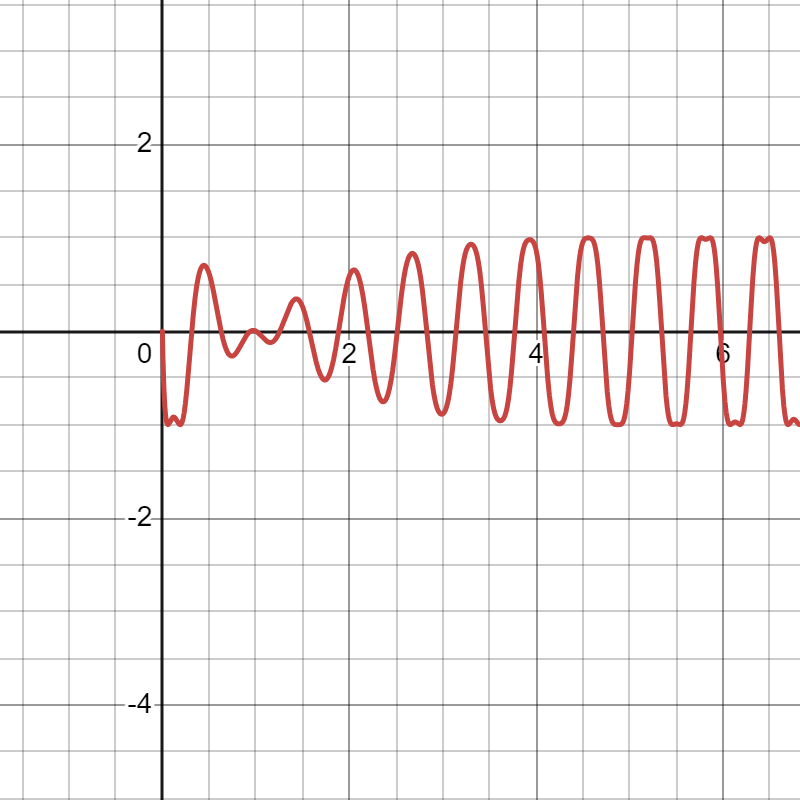
\includegraphics[width=0.5\textwidth]{figures/graph_hardsin.png}
    \caption{График функции $f(x) = \sin\left(\ln(x^{\sin(10x)})\right)$}
    \label{fig:hardsin_graph}
\end{figure}
\end{frame}


\begin{frame}
    \frametitle{Подбор метрики, настройка гиперпараметров}
    \begin{itemize}
        \item \textbf{Функция потерь:}
        \begin{itemize}
            \item Использована среднеквадратичная ошибка (MSE):
            \[
            \text{MSE} = \frac{1}{n} \sum_{i=1}^{n} (y_i - \hat{y}_i)^2
            \]
            \item MSE минимизирует крупные отклонения и стабилизирует сходимость.
        \end{itemize}
        \item \textbf{Гиперпараметры модели:}
        \begin{itemize}
            \item \textbf{Количество слоёв}: 5, \textbf{нейронов в слое}: 30.
        \end{itemize}
        \item \textbf{Оптимизатор:}
        \begin{itemize}
            \item Выбран \textit{Adam}, который стабилизирует градиентный спуск и адаптирует скорость обучения.
            \item Эффективен для временных последовательностей и рекуррентных сетей.
        \end{itemize}
    \end{itemize}
\end{frame}



\begin{frame}
    \frametitle{Экспериментальное исследование}
    \begin{itemize}
        \item \textbf{Цель эксперимента:}
        \begin{itemize}
            \item Сравнить рекуррентные и полносвязные сети на задачах аппроксимации функций.
            \item Оценить время обучения, значение функции потерь (лосс) и качество аппроксимации.
        \end{itemize}

        \item \textbf{Условия эксперимента:}
        \begin{itemize}
            \item Архитектура:
            \begin{itemize}
                \item Количество слоёв: 5.
                \item Количество нейронов в слое: 30.
            \end{itemize}
            \item Количество эпох: 100, 200, 500, 1000 (тестирование на разных значениях).
        \end{itemize}

        \item \textbf{Набор данных:}
        \begin{itemize}
            \item Использованы встроенные функции DEGANN и функция \texttt{hardsin}.
            \item \texttt{hardsin} была выбрана из-за её сложной математической структуры, которая делает её трудной для аппроксимации.
            \item Набор данных позволяет объективно оценить возможности архитектур для задач аппроксимации.
        \end{itemize}

    \end{itemize}
\end{frame}


\begin{frame}
    \begin{itemize}
            \item \textbf{Исследовательские вопросы:}
        \begin{description}
            \item[RQ1:] Способна ли рекуррентная сеть лучше аппроксимировать встроенные функции DEGANN по сравнению с полносвязной?
            \item[RQ2:] Насколько значительна разница в точности аппроксимации и скорости обучения?
        \end{description}
        \item \textbf{Итоги:}
        \begin{itemize}
            \item Эксперимент находится на этапе тестирования.
            \item Полные результаты анализа будут готовы на завершающем этапе работы.
        \end{itemize}
    \end{itemize}
\end{frame}


\begin{frame}
    \frametitle{Результаты аппроксимации функции hardsin}
    \begin{columns}
        \begin{column}{0.5\textwidth}
            \centering
            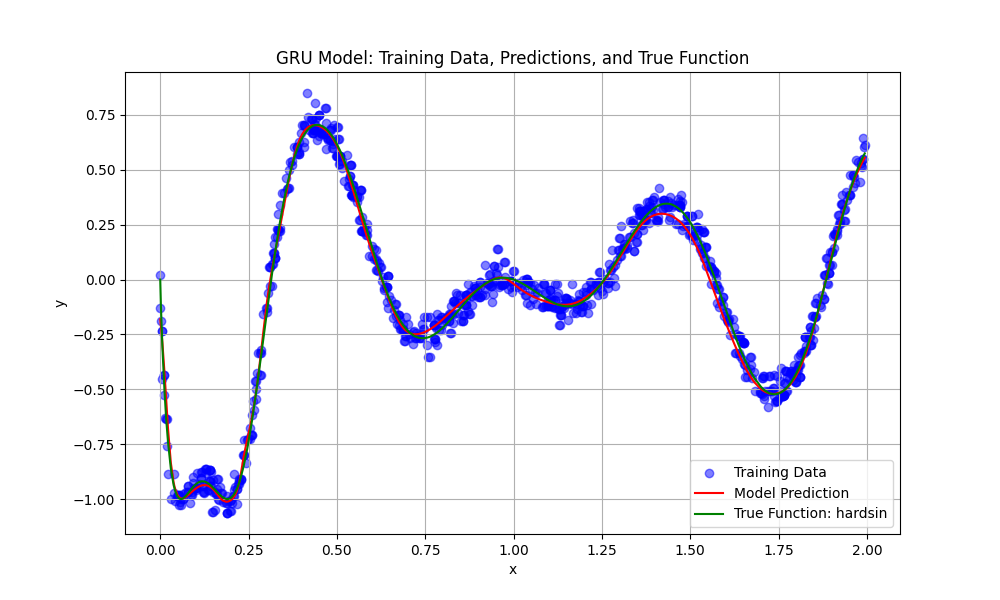
\includegraphics[width=1.1\textwidth]{figures/hardsin_500eph_gru_apr_plot.png}
        \end{column}
        \begin{column}{0.5\textwidth}
            \centering
            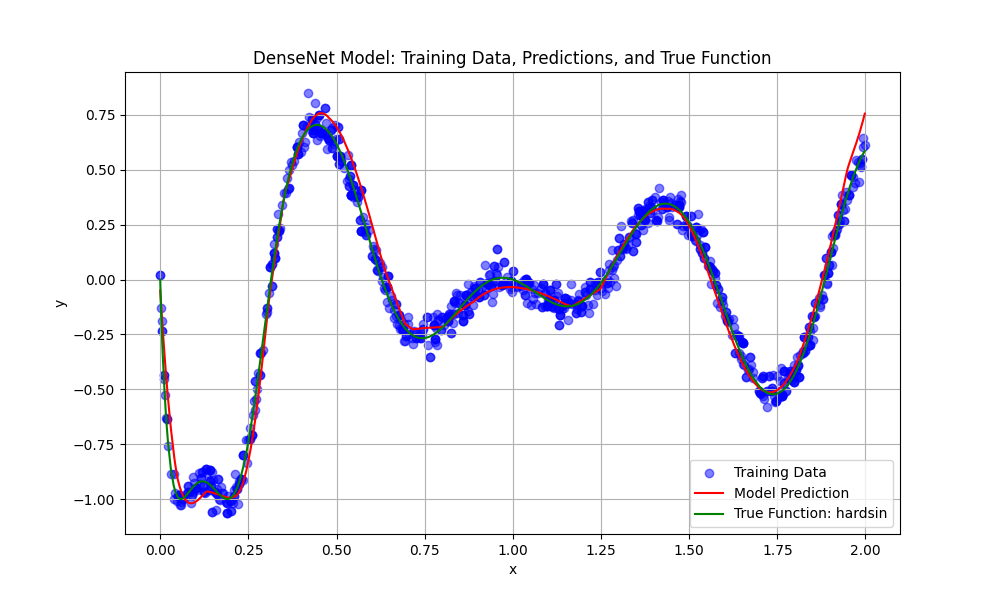
\includegraphics[width=1.1\textwidth]{figures/hardsin_500eph_dense_apr_plot.png}
        \end{column}
    \end{columns}
\end{frame}

\begin{frame}
    \frametitle{Результаты аппроксимации функции hardsin}
    \begin{columns}
        \begin{column}{0.5\textwidth}
            \centering
            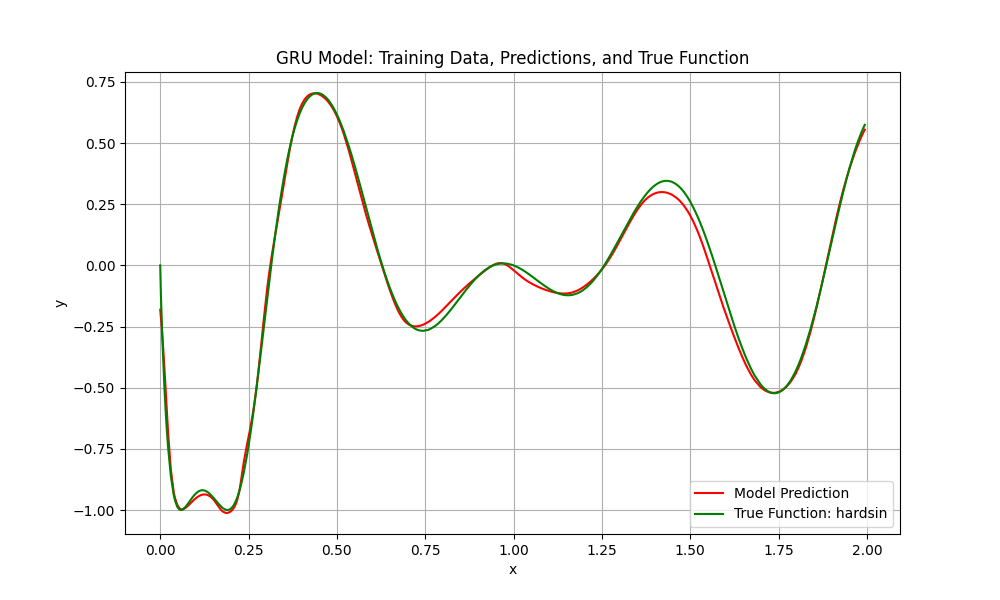
\includegraphics[width=1.1\textwidth]{figures/ch_hardsin_500eph_gru_apr_plot.png}
        \end{column}
        \begin{column}{0.5\textwidth}
            \centering
            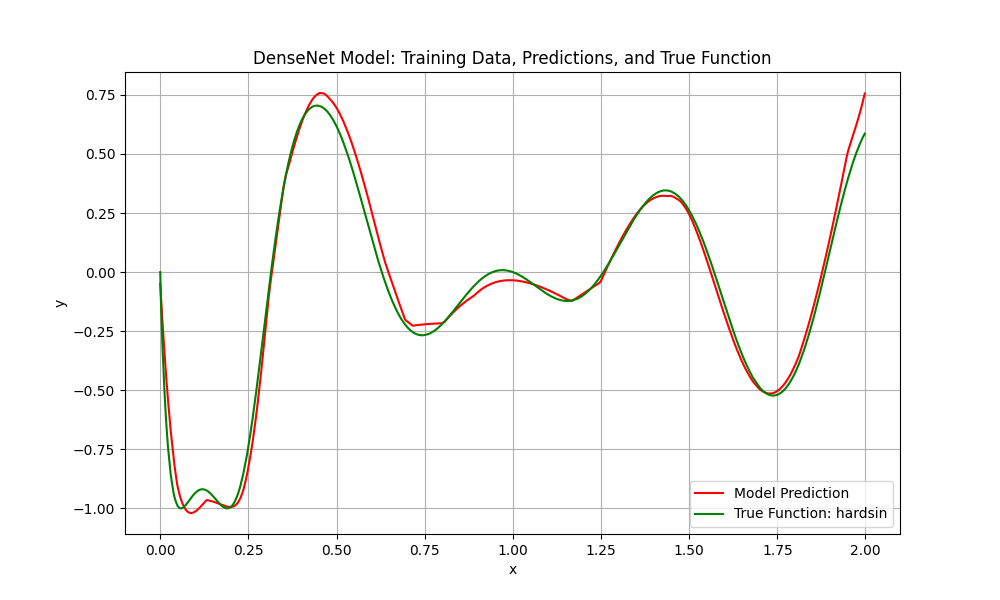
\includegraphics[width=1.1\textwidth]{figures/ch_hardsin_500eph_dense_apr_plot.png}
        \end{column}
    \end{columns}
\end{frame}


\begin{frame}
    \frametitle{Результаты}
    \begin{itemize}
        \item Разработан и реализован модуль с топологией рекуррентной сети для архитектуры GRU, интегрированный в библиотеку DEGANN.
        \item Создана модель с архитектурой GRU, включающая следующие callback-функции:
        \begin{itemize}
            \item Раннее прекращение обучения.
            \item Сохранение лучшей модели.
            \item Визуализация результатов обучения.
        \end{itemize}
        \item Подготовлены специальные датасеты для тестирования, включая сложно-аппроксимируемую функцию \texttt{hardsin}. Реализовано добавление шума для повышения устойчивости модели.
        \item Проведён подбор функции потерь (MSE) и настройка гиперпараметров, обеспечившая баланс между качеством аппроксимации и вычислительными затратами.
    \end{itemize}
\end{frame}


\begin{frame}
    \frametitle{Предстоящие работы}
    \textbf{Предстоящие работы и планы:}
        \begin{itemize}
            \item Работа с экспериментами и более глубокий анализ результатов пока находятся на стадии тестирования.
            \item Планируется разработать кастомную реализацию слоёв GRU для расширения функционала DEGANN.
            \item Продолжить тестирование модели на дополнительных наборах данных.
        \end{itemize}
    \end{frame}

\end{document}

%\begin{frame}[t]
%    \frametitle{Экспериментальное исследование}
%    Постановка эксперимента
%    \begin{itemize}
%        \item На каком наборе данных проводилось экспериментальное исследование, почему были выбраны именно эти данные
%        \item На каком оборудовании проводилось исследование
%        \item Какие решения были выбраны для сравнения и почему
%    \end{itemize}
%\end{frame}
%
%\begin{frame}[t]
%    \frametitle{Результаты экспериментального исследования}
%    \begin{itemize}
%        \item Какие результаты показало экспериментальное исследование
%        \item Желательно привести графики, иллюстрирующие полученные результаты
%              \begin{itemize}
%                  \item У иллюстраций должны быть подписи, у графиков~--- легенда, подписи к осям, например:
%              \end{itemize}
%    \end{itemize}
%    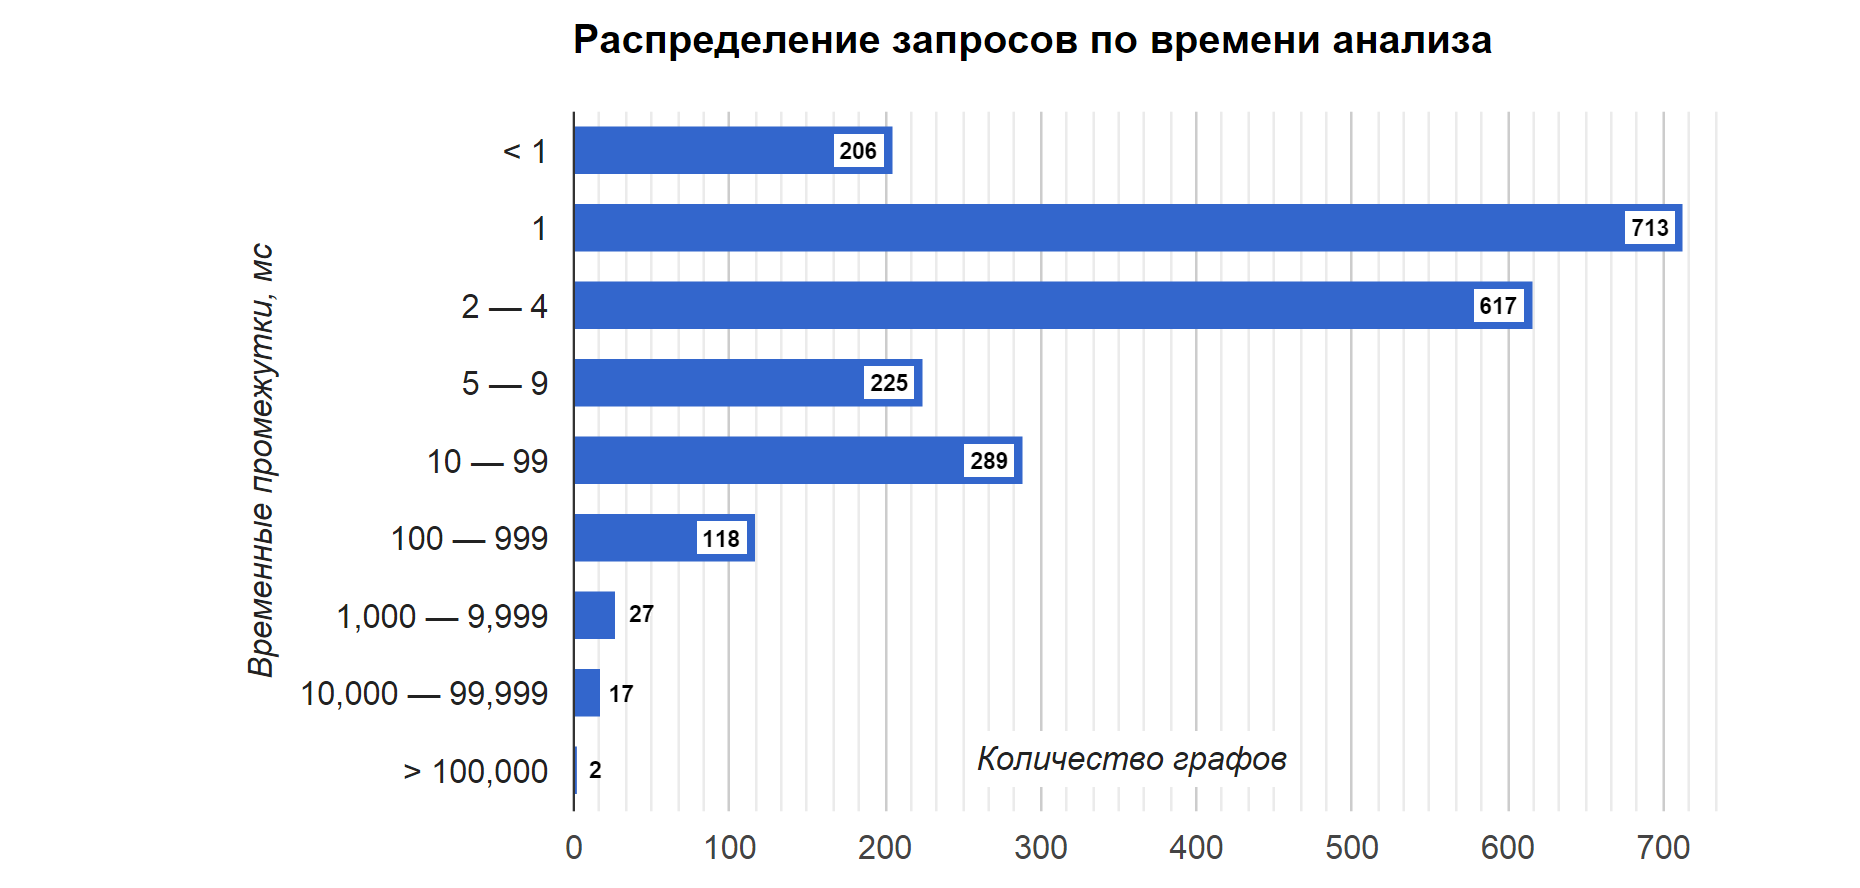
\includegraphics[width=13cm]{figures/dist.png}
%\end{frame}
%
%\begin{frame}
%    \frametitle{Результаты}
%    \begin{itemize}
%        \item Практически то же, что и на слайде с постановкой задачи, но в совершенной форме~--- что делал лично автор
%        \item Четкое отделение результатов своей работы (особенно для коллективных работ)
%        \item Формулировать глаголами совершенного вида в прошедшем времени (\enquote{сделано}, \enquote{получено})
%        \item Обсуждение (ограничения, валидность, альтернативы)
%        \item Не нужно слайдов типа \enquote{Все}, \enquote{Вопросы?}, \enquote{Спасибо за внимание}
%    \end{itemize}
%
%    \begin{itemize}
%        \item Если результаты были представлены на конференции и опубликованы, это желательно указать
%    \end{itemize}
%\end{frame}
%
%%\addtocounter{framenumber}{1}
%\appendix
%
%\begin{frame}
%    \frametitle{Дополнительный слайд}
%    Например, с огромной страшной формулой всего, которая нужна для пояснения деталей при ответе на частый вопрос
%
%    \begin{align*}
%        \MoveEqLeft \lim_{\bigtriangleup t \to 0^+}\int_{\bigtriangleup t}^{T} \! \int_{\Omega} \! D(t_1,x) \frac{\varphi(t_1-\bigtriangleup t,x)-\varphi(t_1,x)}{(-\bigtriangleup t)} \, \mathrm{d}x \, \mathrm{d}t_1 \\
%        &= \lim_{\bigtriangleup t \to 0^+} \int_{0}^{T} \! \int_{\Omega} \! D(t_1,x) \frac{\varphi(t_1-\bigtriangleup t,x)-\varphi(t_1,x)}{(-\bigtriangleup t)} \chi_{(\bigtriangleup t,T)}(t_1) \, \mathrm{d}x \, \mathrm{d}t_1 \\
%        &=\int_{0}^{T} \! \int_{\Omega} \! D(t_1,x) \frac{\partial \varphi}{\partial t_1} (t_1,x) \, \mathrm{d}x \, \mathrm{d}t_1
%    \end{align*}
%\end{frame}
%
%\begin{frame}
%    \frametitle{Второй дополнительный слайд}
%    \begin{itemize}
%        \item Много дополнительных слайдов не надо: 1--2~вполне достаточно в большинстве случаев
%        \item Кроме формул здесь могут быть схемы, рисунки, таблицы и другие вспомогательные материалы
%    \end{itemize}
%
%\end{frame}
%
%\end{document}
%
%
%
%
%
%
%
%
%
%\begin{frame}{Введение}
%    \begin{itemize}
%        \item Дифференциальные уравнения широко применяются в науке и технике (физика, биология, экономика).
%        \item Традиционные численные методы часто сталкиваются с ограничениями по времени вычислений и точности.
%        \item DEGANN — библиотека для нейросетевой аппроксимации дифференциальных уравнений, но она ограничена полносвязными сетями.
%        \item Цель работы: интеграция архитектуры GRU для улучшения точности и производительности в DEGANN.
%        \item GRU эффективны благодаря использованию элементов управления потоком данных (обновление и сброс).
%    \end{itemize}
%\end{frame}
%
%\begin{frame}{Постановка задачи}
%    \textbf{Цель:} Расширение функциональности DEGANN путём интеграции архитектуры GRU.\\
%    \vspace{0.5cm}
%    \textbf{Задачи:}
%    \begin{itemize}
%        \item Разработать модуль для интеграции GRU с TensorFlow.
%        \item Реализовать модель и callback-функции для отслеживания и улучшения обучения.
%        \item Создать сложно-аппроксимируемую функцию и провести обучение модели.
%        \item Настроить гиперпараметры, метрики и оценить производительность GRU.
%    \end{itemize}
%\end{frame}
%
%\begin{frame}{Обзор существующих решений}
%    \begin{itemize}
%        \item RNN:
%        \begin{itemize}
%            \item Учитывают временные зависимости, но страдают от затухания/взрывов градиентов.
%        \end{itemize}
%        \item GRU:
%        \begin{itemize}
%            \item Упрощённая версия LSTM с меньшим числом параметров.
%            \item Использует обновляющий и сбрасывающий гейты для долгосрочной памяти.
%        \end{itemize}
%        \item TensorFlow:
%        \begin{itemize}
%            \item Поддержка готовых слоёв GRU (tf.keras.layers.GRU), что упрощает реализацию.
%        \end{itemize}
%    \end{itemize}
%\end{frame}
%
%\begin{frame}{Архитектура решения}
%    \begin{itemize}
%        \item Реализация класса \textbf{TensorflowGRUNet}, интегрированного в DEGANN через IModel.
%        \item Основные параметры:
%        \begin{itemize}
%            \item \texttt{input\_size}, \texttt{block\_size}, \texttt{output\_size}.
%            \item Dropout для предотвращения переобучения.
%        \end{itemize}
%        \item Callback-функции:
%        \begin{itemize}
%            \item Раннее прекращение обучения, визуализация потерь, сохранение лучшей модели.
%        \end{itemize}
%    \end{itemize}
%\end{frame}
%
%\begin{frame}{Экспериментальное исследование}
%    \textbf{Условия эксперимента:}
%    \begin{itemize}
%        \item Датасет: функция \texttt{hardsin}, сложная для аппроксимации.
%        \item Шум добавлен для повышения устойчивости модели.
%    \end{itemize}
%    \textbf{Метрики:}
%    \begin{itemize}
%        \item Среднеквадратичная ошибка (MSE).
%    \end{itemize}
%    \textbf{Результаты:}
%    \begin{itemize}
%        \item GRU показала лучшую стабильность и точность по сравнению с полносвязными сетями.
%        \item Визуализация результатов показывает хорошую аппроксимацию функции.
%    \end{itemize}
%\end{frame}
%
%\begin{frame}{Заключение}
%    \begin{itemize}
%        \item Разработан и интегрирован модуль GRU в DEGANN.
%        \item Реализованы callback-функции для улучшения обучения.
%        \item Проведён эксперимент, подтвердивший эффективность GRU для задач аппроксимации.
%        \item Код доступен в репозитории DEGANN.
%    \end{itemize}
%    \textbf{Планы:} изучение других архитектур (например, LSTM) для дальнейшего расширения функционала DEGANN.
%\end{frame}